\section{Implementation}
\label{sec:implementation}

In this section, we describe the implementation details of \system.
The implementation consists of two components: data plane and user space tools. 
The data plane was implemented in the NetFPGA SUME platform~\cite{SUME2014}.
The user space tools are composed of a controller responsible for defining how the data plane will forward the packets, and software to configure the data plane features, according to the user-created C and P4 programs.


\subsection{Hardware Instance}

FPGA (Field Programmable Gate Array) enables to build hardware logic system.
%In this work, eBPFlow was implemented in NetFPGA SUME platform. 
The NetFPGA SUME hardware has four SFP+ transceivers that support 10 Gbps Ethernet ports.
It connects to a motherboard through an PCIe Gen 3 x8 adapter.
It contains a Xilinx Vertex-7 690T FPGA~\cite{Virtex7},
which has approximately 693,120 logic cells, a 27 MiB SRAM and 5 ns (200 MHz) clock cycle.
%\marcos{XXXX logic cells, a 4 KiB SRAM with $2^{19}$ lines and 8 ns (125 MHz)} clock cycle.

\textcolor{black}{The packets in the NetFPGA are processed in the form of 256-bit words and 128 bits control to identify the word type (data or metadata). Words are transmitted by the data signal and control. If control signal is zero, it means that the words of the packet are being transmitted, otherwise the words are from the metadata.}

%The packets in the NetFPGA are processed in the form of 64-bit words and 8-bit control to identify the word type (data or metadata). Words are transmitted by the data signal and the control by the ctrl signal. If the cntrl signal is zero, it means that the words of the packet are being transmitted, otherwise the words are from the metadata.

%The NetFPGA processes up to 64 bits of packet data per clock cycle (8 ns). Considering a packet size of 1,500 bytes and with that cycle, a packet takes approximately 2 $\mu{s}$ to be processed.

%The standard NetFPGA library provides the following modules: input arbiter, output port lookup and output queue. The input arbiter receives the packets from the network (via the MAC interface) or the PCI bus (via CPU) in the format of 64-bit words and stores them in internal queues of the module. Then, the words are taken from the queues using the round-robin algorithm, and it routes them to the output port lookup module.  The output port lookup module is responsible for defining which port the packet will be sent based on the packet properties, for example, an input port or destination address. The outgoing port of all incoming packets is configured in the metadata output port field. We implemented the device functionalities in the output port lookup module.

The standard NetFPGA library provides the following modules: input arbiter, output port lookup and output queue. The input arbiter receives the packets from the network (via the MAC interface) or the PCI bus (via CPU) in the format of 256-bit words and stores them in internal queues of the module. Then, the words are taken from the queues using the round-robin algorithm, and it routes them to the output port lookup module.  The output port lookup module is responsible for defining which port the packet will be sent based on the packet properties, for example, an input port or destination address. The outgoing port of all incoming packets is configured in the metadata output port field. We implemented the device functionalities in the output port lookup module.

\textcolor{black}{Table \ref{tab:eBPFresource} lists the logic and memory resource used by eBPFlow implementation on NetFPGA SUME.  We compared the resource used by eBPFlow with a reference switch.}      

\begin{table}[tb]
\centering
\caption{NeFPGA's resource requirements for eBPFlow compared to reference switch.}
\label{tab:eBPFresource}
\begin{tabular}{|c|c|c|}
\hline
\textbf{Resource Type} & \textbf{Reference switch} & \textbf{eBPFlow} \\ \hline
\# Slice LUTs          & 49436 (11\%)              & 54085 (12.48\%)  \\ \hline
\# Block RAMs          & 194 (13\%)                & 200.50 (13.63\%) \\ \hline
\end{tabular}
\end{table}

After synthesis, eBPFlow consumed 11.76 \% of logical slice and 8.18 \% of the register slice on NetFPGA SUME. The maximum frequency is 185.83 MHz (cycle of (5.405 ns).

\subsection{Finite State Machine of HW Controller}

The finite state machine (FSM) in the module output port lookup controls the whole operation of packet processing. It removes the packet from the internal queue of the module (forwarded by the input arbiter module), starts executing the eBPF instructions and forwards the packet to the next module (action packet) when the last instruction (\texttt{exit}) of eBPF is executed. The finite state machine is made up of eight states.

\subsection{eBPF Processor}

\begin{figure*}[t]
\centering
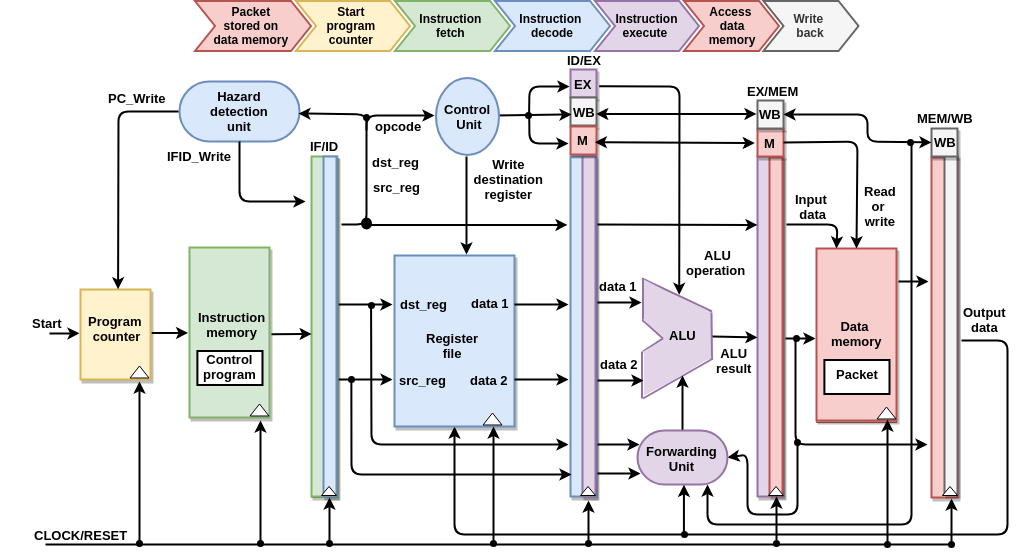
\includegraphics[width=.9\textwidth]{figures/06_fig02.png}
\caption{Control and Datapath of the eBPF processor.}
\label{fig:06_fig02}
\end{figure*}


The eBPF processor is responsible for performing the parse, matching, and actions according to the user-created user-generated C-code or P4-generated eBPF instructions. When starting the operation of the device, the user must load the eBPF instructions into the instruction memory to define  the behavior of the data plane.
% After the instructions have been loaded the switch starts processing the packets.

Figure~\ref{fig:06_fig02} presents the data and control path in register transfer level (RTL), containing five data functional units (program counter, instruction memory, register file, arithmetic logic unit (ALU), data memory) and three control units (hazard detection, forwarding, and control).

After the instruction is fetched from the memory instruction, it is divided into five parts: operation code, destination and source register address, offset, and immediate value. Each part of the instruction is sent to a specific unit. The control unit receives the operation code and forwards the control signals to the functional units, defining the behavior of each unit. For example, instructions in the ALU (arithmetic and logical unit) class do not use the data memory, so the read and write signals from the data memory are not activated.

The eBPF opcode is divided into seven classes: immediate load, load, immediate store, store, arithmetic and logical operations, jumps, 64-bit arithmetic and logical operations, and the other class is reserved for future use. The eBPF processor has 64-bit instruction, 32 bits for representing an immediate number (\texttt{imm}), 16 bits for offset, 4 bits for source register, 4 bits for destination register and, finally the 8-bit operation code (\texttt{opcode}). The opcode can be redivided depending on the instruction class. For load and store, the opcode has 3 most significant bits for memory access mode, 2 bits for word size and 3 bits for instruction class. For the jump instructions, logic and arithmetic, the 4 most significant bits specify what the operation is, 1 bit to specify whether the instruction is performed with the immediate value or with the source operand and, finally 3 bits less significant for the instruction class.

\begin{table}[tb]
\centering
\caption{Description of the eBPF register set.}
\label{tab:eBPFreg}
\begin{tabular}{|c|l|}
\hline
\textbf{Register} & \textbf{Description} \\
\hline \hline
R0 & return value from function, and exit value\\
\hline
R1 - R5 & arguments from eBPF program to function\\
\hline
R6 - R9 & callee saved registers that function preserve\\
\hline
R10 & read-only frame pointer to access stack\\
\hline
\end{tabular}
\end{table}

Read and write data operations in the registers are performed in the register file. 
In the read operation, the register file receives the addresses of the destination\/origin register and forwards the data referring to the ALU addresses. The write operation in the register file is performed after reading the data in the data memory or an ALU operation.
Table~\ref{tab:eBPFreg} describes the functionality of each eBPF register.

% Therefore, eBPF calling convention is defined as:
%
%    * R0	- return value from in-kernel function, and exit value for eBPF program
%    * R1 - R5	- arguments from eBPF program to in-kernel function
%    * R6 - R9	- callee saved registers that in-kernel function will preserve
%    * R10	- read-only frame pointer to access stack


The ALU of the eBPF processor is capable of performing arithmetic and logic operations based on the signal sent by the control. The ALU result can be forwarded as the data memory address or as the write data of the destination register in the register file.

The data memory has the functionality of storing metadata and packet words for the eBPF processor to perform the actions in the packet according to the eBPF instructions. There were two design options to implement the data memory: as register or at SRAM. Implementing the data memory as register has a delay of only 1 cycle in accessing it but consumes logical cells. The option of using SRAM does not consume logical cells but has a delay of 4 cycles. Since accessing the data memory is a critical operation, we opted to implement the data memory as a register file. The size of the data memory of the eBPF processor has a capacity of up to 256 words of 64 bits. With this capability, one metadata and one packet of up to 1,500 bytes can be stored. 
%We currently define the data memory with this capacity because of the little logical resource (53,000 logical cells) available in the NetFPGA SUME. 
The write operation is synchronous (only happens at clock edge) and the read operation is asynchronous.

The eBPF processor has a set of read and write instructions in the data memory with the following size types: 8 bits (byte (B)), 16 bits (half-word (H)), 32 bits (\ textit {word} (w)), and 64 bits (double word (DW)). In order to be able to read and write data of these size types, 
we add decoders and a control signal from the control unit to the decoders. The decoders perform the data mapping according to the control signal.
We also have to use the generate-for construct available by Xilinx tool. 
This construct does a loop unrolling before synthesizing the code and enables creating variable data size memory.

%We initially projected the eBPF processor for single-cycled datapath. Later, we extend it to a 5-stage pipeline:
We design the eBPF processor with a 5-stage pipeline: instruction fetch (IF), instruction decode (ID), execute (EXE), memory (MEM), and write back (WB).
IF stage gets instruction from memory and increments program counter (PC).
ID stage translates opcode into control signals and reads registers from the register file. EXE stage performs ALU operation, and computes jump/branch targets. MEM stage accesses data memory if needed. WB stage updates register file. 
This design follows the MIPS load-store pipeline architecture~\cite{Hennessy:2011:CAF:1999263}.
We add four pipelined registers (between the stages), the forwarding unit, and hazard unit. 

The forwarding unit is designed to solve the data hazards at ALU in a pipelined processor. The correct data at the output of the ALU is forwarded to the input of the ALU when data hazards are detected. These hazards are detected when the source register of the current instruction is the same as the destination register of the previous instruction.

The hazard detection unit is projected to solve data and control hazards. When data hazards occur, it needs to delay 1 cycle before forwarding.
Data hazard stalls 1 cycle when the destination register of the current instruction is the same as the source register of the coming instruction in ID stage. The control hazard happens when there is a jump/branch. In this case, the hazard detection unit discards instructions in IF and ID stages.
These units are implemented with logic gates to minimize latency.
Thus, we design an eBPF processor with a pipeline of 5 stages.


\subsection{Instruction Memory} 

%The eBPF instructions define the behavior of how the eBPF processor handles the packets. The instructions are inserted into the instruction memory via the NetFPGA register interface. Software registers were created to insert the eBPF instructions into the processor instruction memory. The instructions are received on the switch through messages sent by the controller. The instructions are then written to the software registers and forwarded to instruction memory via the hardware PCI bus.

%As a design decision, we have put the instruction memory outside of the eBPF processor in order to enable the connection of multiple processors in the future using a shared instruction memory. By increasing the number of eBPF processors in the datapath of the switch, more packets can be processed, contributing to the increase in the switch's throughput.

The eBPF instructions define the behavior of how the eBPF processor handles the packets. The instructions are inserted into the instruction memory via the NetFPGA register interface. Software registers were created to insert the eBPF instructions into the processor instruction memory. The instructions are received on the network element through messages sent by the controller. The instructions are then written to the software registers and forwarded to instruction memory via the hardware PCI bus.

\textcolor{black}{Instruction memory uses a double buffer system - DBS (Figure~\ref{fig:mem_db}) to provide zero downtime in the change of eBPF programs. This system is composed of two memories (M$_{1}$ and M$_{2}$). Both memories never assume the same state (writing or reading) at the same time. It means that while eBPF program is written to a memory, the eBPF processor reads the instructions of the other memory. DBS is initialized with eBPF instructions written on M$_{1}$, while M$_{2}$ remains idle. The system remains in the wait state until a new set of instructions will be received. After the instructions are written to M$_{1}$, the system will return to the standby state. When a new set of instructions is received, the memories change their states, which means that M$_{1}$ will no longer be written and will be read while M$_{2}$ will be written. If a new instruction set is received, these instructions are written in M$_{2}$, while the instructions previously written in M$_{1}$ are read and processed by the eBPF processor. This process can be repeated indefinitely.} 

\begin{figure}[tb]
\centering
\includegraphics[width=\linewidth]{figures/memory_db.png}
\caption{Instruction memory - Double Buffer System.}
\label{fig:mem_db}
\end{figure}

\textcolor{black}{As a design decision, we have put the instruction memory outside of the eBPF processor in order to enable the connection of multiple processors using a shared instruction memory. By increasing the number of eBPF processors, more packets can be processed, contributing to the increase in the throughput.}


\begin{comment}
%The eBPF instructions define the way in which the eBPF processor will process the packages. Instruction memory was implemented with a double buffer system in order to provide zero downtime in the prototype through important changes, such as sudden changes in the packet processing pattern. 

%The implementation of the double buffer memory started from the following design decision: the memories involved, M1 and M2, will never assume the same state (of writting or reading) at the same time. It means that while data is written to a memory, data is read from the other one and vice versa. 
%From this definition, we implemented an efficient management system that works as follows: the first memory to be written will always be M1, while M2 will remain idle. 
%The system remains in the wait state until a new set of instructions is received. Writing in M1 is initiated when a set of instructions is received. 
%Once all instructions are written to M1, the system will return to the standby state. When a new set of instructions is received, the memories will have their states changed, what means that M1 will no longer be written and will be read while M2 will be written. The new instruction set is then written in M2, while the instructions previously written in M1 are read and processed by the eBPF processor. This process is repeated indefinitely until the instruction sets are no longer received. In this case, the last written memory has its state maintained, that is, the state of write and read of the memories is only changed upon receipt of a new set of instructions. 
\end{comment}




\subsection{Maps}
\label{ssec:maps}

eBPF Linux kernel implementation allows for maps. Maps are a generic data structure that store different types of data in the form of key-value pairs. 
% Currently, the Linux Kernel allows for three different types of maps. Hash map applies a hash before inserting in the table. Array map accesses the table with an integer index. Program array map is used to store a program. eBPF programs can manipulate maps through specific kernel function calls, such as bpf\_map\_lookup\_elem().

In our design, we currently provide three types of maps: longest prefix matching (LPM), exact-match, and array map, which are provided in eBPFlow as hardware components. For LPM, we use the Ternary Content Addressable Memory (TCAM) module combined with the BRAM (Block RAM). TCAM is a specialized high-speed memory that does LPM searches very fast (1 cycle). TCAM uses three different inputs: 0, 1,  and "don't care". There is also the unmatchable (U) option provided by Xilinx design~\cite{xilinx_IP_2018} but we did not use it. Our TCAM module spends 16 cycles for a write operation and only 1 cycle for a read operation. For the exact-match, we use the Content Addressable Memory (CAM) module combined with the BRAM. For the array map, we use the DRAM memory.

The TCAM is implemented using Xilinx SRL16e primitives~\cite{xilinx_kylelocke2011}.
It is generated using Xilinx's IP core generator \textit{coregen}~\cite{xilinx_core_generator_2018}. The CAM is implemented using block RAM (BRAM) instead of SRL16e. This option enables to write on CAM using 2 cycles instead of 16 cycles.

There are three functions to manipulate the maps: update, delete, and lookup. The update operation updates an item into the map. If the item does not exist, it inserts the item. The delete operation removes the item with the given key. The lookup operation searches for the key and returns an item.
To manipulate these tables, the user can write C program and invoke the three functions through function calls.

\begin{figure}[tb]
\centering
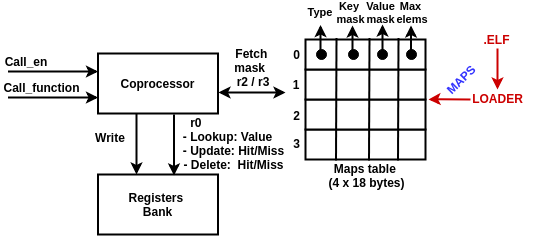
\includegraphics[width=1.\linewidth]{figures/coprocessor.png}
\caption{Coprocessor and Maps table.}
\label{fig:coproc}
\end{figure}

\textcolor{black}{
Since maps are generic data structures, allowing keys and values of multiple byte lengths, the coprocessor needs to know the actual size of the data being read/written to map memory. This information is stored in a \textit{maps table}, shown in Figure \ref{fig:coproc}, which holds metadata about each map declared in the current loaded program. This includes map type, key, value masks, and the maximum number of elements allowed in the map. 
%Our current implementation allows for maximum key and value sizes of 6 and 4 bytes, respectively.
The values are passed to the coprocessor by copy through registers R1-R4 on map calls. A lookup on the maps table is performed on every map operation to retrieve key and value masks, which are used in a bitwise-AND operation with the data to clean any unwanted bits. The map's type is also used by the coprocessor to switch to the proper memory unit (CAM or TCAM).
}

\subsection{Call instruction}

%eBPF allows invoking functions to access tables.
% The function calls are used to manipulate maps.
% In the Linux kernel, the software implementation of call functions is straightforward.
% There is a function pointer table. It registers the function call in the function pointer table.
% The call instruction is implemented as a function invocation thought the function pointer table.
% Parameters are passed through register 1 to 5. 

% The hardware call instruction implementation is different. It has to save the program counter (PC) value at the stack. It can pass parameters through registers or through the stack. Then, the processor executes an absolute jump to where the function instructions are located. 
eBPF allows invoking functions to access tables.
In our design, to manipulate maps, we opted to use the TCAM, CAM, and DRAM modules.
Thus, to manipulate tables, the function call inside the processor is replaced by a communication to the coprocessor hardware module. 
Thus, where there is call instruction, the processor communicates with the coprocessor module.
This module identifies what function (lookup, update, delete) was called though the call instruction immediate opcode parameter. 
Parameters are passed through register 1 to 4.
Register R1 indicates which hardware module to communicate (tables TCAM, CAM, DRAM, respectively).
Register R2 provides the key.
Register R3 stores the item.
Register R4 has the TCAM mask item.
Function return parameter is through register R0.
Since the call instruction requires register values, it can also suffers from hazard in the pipeline. The hazard unit has to stall to solve this issue.
Thus, for optimization, current call instruction is done through synchronous communication with coprocessor hardware modules since their functions are implemented in hardware.




\subsection{Synchronization}

\begin{figure}[tb]
\centering
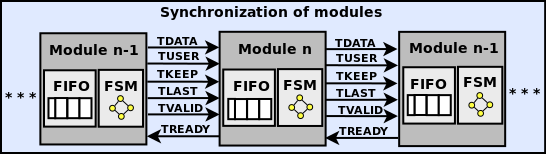
\includegraphics[width=\linewidth]{figures/06_fig04.png}
%\caption{Synchronization of the switch modules.}
\caption{Synchronization of the eBPFlow modules.}
\label{fig:06_fig04}
\end{figure}

\begin{comment}
The synchronization of the NetFPGA modules operates in a standardized way. Figure~\ref{fig:06_fig04} shows the synchronization of modules with their respective signals. The write (wr) and ready (rdy) signals control the communication between the modules. The wr signal informs when the previous module is ready to transmit (when it has content to transmit) and the rdy signal indicates that the next module is ready to receive. The transfer of data between modules only occurs if the two signals are active.

Each module contains an input queue and a finite state machine. The input queue is used to temporarily store the \textit{data} and \textit{ctrl} signal until the state machine module can remove the word from the queue. The state machine of each module has a specific behavior.
\end{comment}

\textcolor{black}{The synchronization of the NetFPGA modules operates of standardized way based on AXI-4 stream Xilinx protocol~\cite{XilinxAXI4}. Figure~\ref{fig:06_fig04} shows the 
modules' synchronism with their respective signals. TDATA represents the data stream. TUSER is out of band metadata. TKEEP marks qualified bytes (i.e byte enable). TLAST indicates end of packet/burst. The write (TVALID) and ready (TREADY) signals control the communication between the modules. The TVALID signal informs when the previous module is ready to transmit (when it has content to transmit) and the TREADY signal indicates that the next module is ready to receive. The transfer of data between modules only occurs if the two signals are active.} 

\textcolor{black}{Each module contains an input queue and a finite state machine. The input queue is used to temporarily store the TDATA, TUSER, TKEEP  and TLAST signals until the state machine module can remove the word from the queue. The state machine of each module has a specific behavior.}

\subsection{User space tools}

\color{black}{
The user space tools are composed of the controller and applications created at the user level.
The controller implements the Southbound API defined in \textsection~\ref{sec:southboundAPI}.
It was implemented in Python.
The controller opens a socket connection to the device to exchange the Southbound messages.

The applications to execute over the controller were also implemented in Python.
They open a connection to the controller and transmit the eBPF program, which was already compiled, as bytecodes.
These bytecodes are installed in the hardware by the controller at runtime.
In \textsection~\ref{sec:experiments}, we provide examples of applications.
}

\color{black}{
A set of tools were implemented as part of the eBPFlow infrastructure: an eBPF disassembler, a code loader (\textsection~\ref{ssec:loader}), a software emulator, and a CLI application to interact with the processor.

The emulator leveraged the uBPF\footnote{https://github.com/iovisor/ubpf} GitHub project and aims to replicate the processor's behavior in software. It enables code testing and debugging with well-known tools such as \textit{gdb}, enabling faster and easier bug detection and correction even before deploying the code to hardware.

In addition to these tools, many application examples were also created, as explained in \textsection~\ref{sec:experiments}.
}

\subsection{Loader}
\label{ssec:loader}
Loading code to the processor is done through the use of a \textit{loader}, specially designed for the eBPF processor. It serves two main purposes: modifying the code with processor specifics and interacting with its register interface.

At the beginning of every eBPF program, registers R1 and R10 need to be initialized with pointers to the packet, and to the top of the stack, respectively. Since these are specific to the runtime environment (here, the processor), such initialization is not part of the code generated by \textit{clang} compiler. Thus, when loading a program, the loader appends two instructions at the beginning of the instruction memory to correctly initialize those two registers with the proper addresses. 

To handle maps, the compiler adds map information to the eBPF ELF file as a relocation section, which needs to be processed before code execution. This job is also done by the \textit{loader}, which adjusts all map \textit{call} instructions with their corresponding map values according to the relocation table in the ELF file.

Finally, the \textit{loader} interacts with the processor register interface to load the list of instructions to the instruction memory and metadata about every map in the program to the maps table (\textsection \ref{ssec:maps}), after which the processor is ready to execute any incoming packets based on the loaded eBPF program. Through the register interface, the loader is also able to query status information about the processor, such as the value of R0, which instruction memory is being currently used and if the last load was successful or not.



